\documentclass[11pt,a4paper]{article}
\usepackage[T2A]{fontenc}
\usepackage[utf8]{inputenc}
\usepackage[russian,english]{babel}
\usepackage{amsmath,amssymb,bm}
\usepackage{graphicx}
\usepackage{booktabs}
\usepackage[margin=24mm]{geometry}
\usepackage[hidelinks]{hyperref}
\usepackage{microtype}
\title{Обобщённая динамика и аналитические критерии встречного вращения в мультипольной RF-ловушке}
\author{V17C.14 theory study}
\date{\today}
\begin{document}
\maketitle

\begin{abstract}
Исследуется обобщённая модель взаимодействующих заряженных частиц в двумодовом временно-периодическом мультипольном электрическом поле, с линейным сопротивлением и осесимметричным DC-удержанием. Для leading-only RF усреднения выведены радиальный и тангенциальный дрейфы, найдено локально устойчивое одночастичное встречновращающееся решение для параметров local15, сформулированы точные балансы энергии и момента и построены аналитические приближения для внутренних кольцевых и осевых мод. Один опубликованный V17C.13 N=6 расчёт используется как выбранный ориентир, а не как случайная оценка бассейна. Результат ограничен усреднёнными корнями, frozen-phase матрицами и воспроизведёнными исходными данными: полная Floquet/Lyapunov устойчивость, физическая реализуемость и устойчивое осевое разделение не установлены.
\end{abstract}

\section{Модель}
Введём \(\tau=\Omega_1t\), \(\bm x_i=\bm r_i/R\), \(\mu_i=m_i/m_1\), \(Q_i=q_i/q_1\), \(\lambda_i=\gamma_i/(m_i\Omega_1)\), \(\kappa=q_1^2/(4\pi\varepsilon m_1R^3\Omega_1^2)\) и \(\phi=q_1\Phi/(m_1R^2\Omega_1^2)\). Уравнения для \(N\) центров:
\begin{align}
\bm x_i'&=\bm u_i,\\
\mu_i\bm u_i'&=-Q_i\nabla\phi(\bm x_i,\tau)-\mu_i\lambda_i\bm u_i+
\kappa\sum_{j\ne i}Q_iQ_j\frac{\bm x_i-\bm x_j}{|\bm x_i-\bm x_j|^3}.
\end{align}
RF-потенциал представлен Fourier--MFS мультипольными компонентами и не отождествляется с амплитудами граничных электродных напряжений. Численный RHS и вариационный Якобиан реализованы в `numerical/generalized_dynamics.py`.

Полная безразмерная энергия и её баланс:
\begin{align}
\mathcal E&=\frac12\sum_i\mu_i|\bm u_i|^2+\sum_iQ_i\phi(\bm x_i,\tau)+\kappa\sum_{i<j}\frac{Q_iQ_j}{d_{ij}},\\
\mathcal E'&=\sum_iQ_i\partial_\tau\phi(\bm x_i,\tau)-\sum_i\mu_i\lambda_i|\bm u_i|^2.
\end{align}
Попарные Coulomb torque взаимно сокращаются в сумме; внешнее RF-поле и сопротивление задают суммарный баланс момента.

\section{Локальное RF-усреднение}
Для медленно меняющегося положения и гармонического ускорения \(\operatorname{Re}[\bm f(\bm X)e^{-i\nu\tau}]\) быстрый отклик линейно затухающей системы равен \(\hat{\bm\xi}=\bm f/(-\nu^2-i\lambda\nu)\). Средняя поправка второго порядка:
\begin{equation}
\overline{\bm F}_{\rm eff}=\frac12\operatorname{Re}\!\left[(D\bm f)\hat{\bm\xi}^{*}\right].
\end{equation}
Для мультипольного поля \(\phi=\operatorname{Re}[a\rho^ne^{i(k\theta-\nu\tau)}]\), \(\sigma=\operatorname{sgn}k\), имеем
\begin{equation}
\overline F_\rho=-K_n\rho^{2n-3},\qquad
\overline F_\theta=\sigma K_n\frac{\lambda}{\nu}\rho^{2n-3},\qquad
K_n=\frac{\alpha^2n^2(n-1)|a|^2}{\nu^2+\lambda^2},\quad \alpha=Q/\mu.
\end{equation}
Усреднённая схема требует малой локальной поправки micromotion и медленного изменения envelope; значение \(\epsilon_\mu=1\) не является универсальным порогом.

\section{Круговые корни local15}
Для противоположных ведущих гармоник \((n,\sigma)=(2,+1),(4,-1)\):
\begin{equation}
\bar\omega(\rho)=K_1-K_2\rho^4/\nu,\qquad
G(\rho)=\bar\omega^2+\alpha\beta-K_1-K_2\rho^4=0,\quad 0<\rho<1.
\end{equation}
Значения local15: \(A=0.03716194907442204\), \(B=0.1626938199343468\), \(\nu=3.1118029452860356\), \(\beta=0.017273303124515367\), \(\lambda_1=0.20975541409005094\), \(\lambda_2=0.12617311138613094\), \(\alpha_1=1\), \(\alpha_2=0.34126014359705537\). Совместное решение даёт \((\rho_1,\bar\omega_1)=(0.5503691530,+0.0014400542)\) и \((\rho_2,\bar\omega_2)=(0.7663818562,-0.0010579232)\). Собственные значения reduced 3D polar Jacobian для обоих корней имеют отрицательные действительные части. Это локальная устойчивость автономной усреднённой одночастичной системы.

Полный MFS+C ориентир V17C.13 имеет group means \(\rho=(0.5480284,0.7660739)\), \(\bar\omega=(+0.0015013354,-0.0009995555)\). Он получен при RK4/96 в выбранном 3+3 старте на 120\,000 RF-периодов после loading. Межмодельные частотные сдвиги порядка 4--6\% не являются контролируемыми численными ошибками.

\begin{figure}[ht]
\centering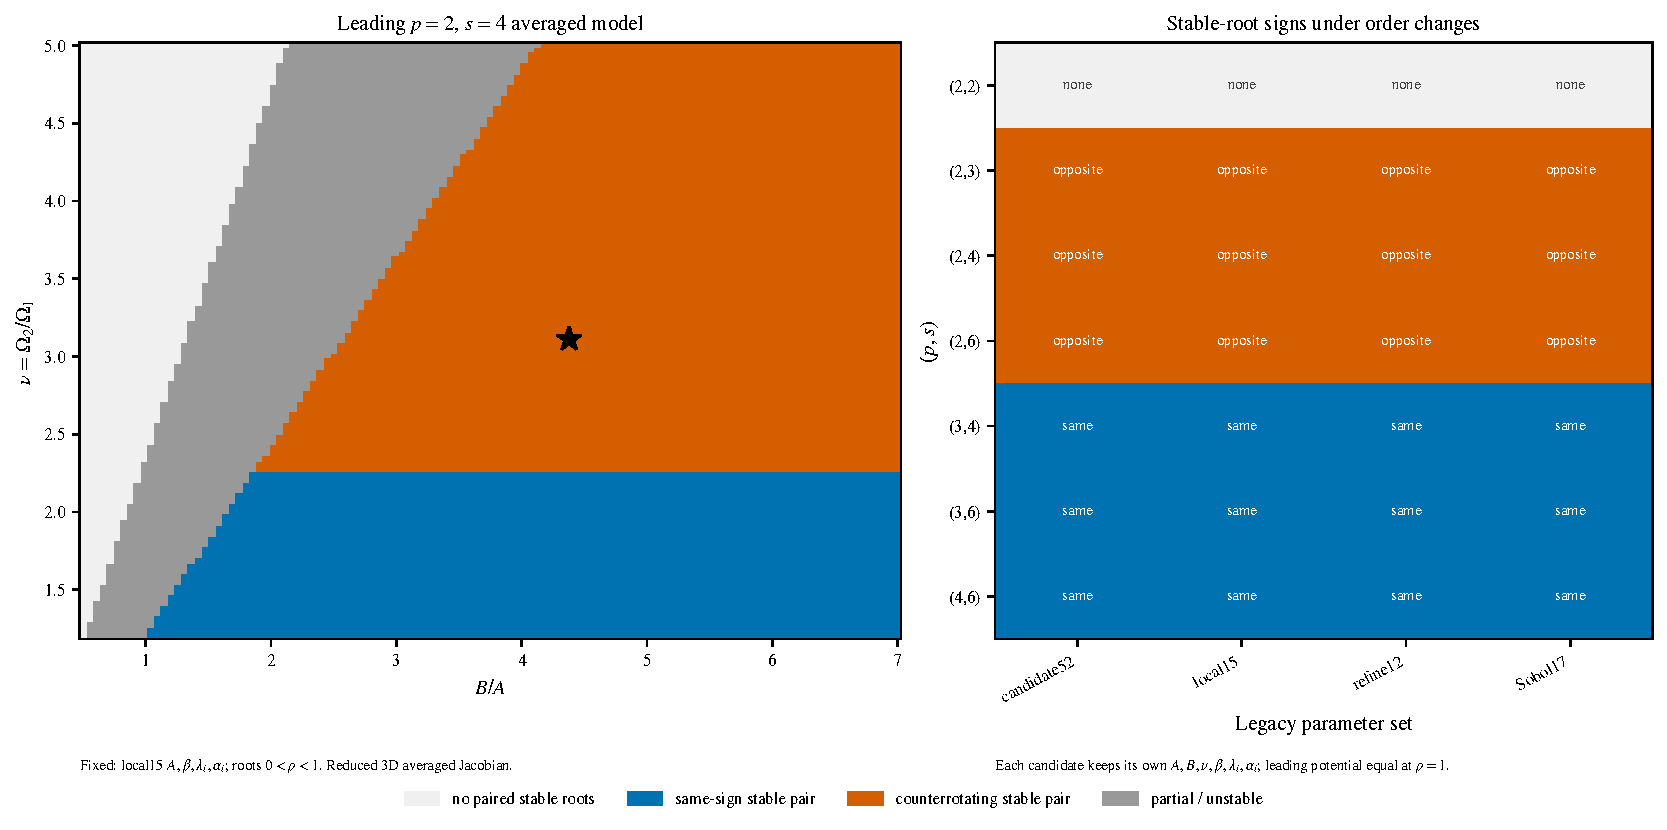
\includegraphics[width=.82\linewidth]{figures/FIG01_ANALYTIC_COUNTERROTATION_MAP.pdf}
\caption{Leading-only map of stable one-particle root signs. Fixed parameters and classification are given in the figure and `FIGURE_AUDIT_RU.md`.}
\end{figure}
\begin{figure}[ht]
\centering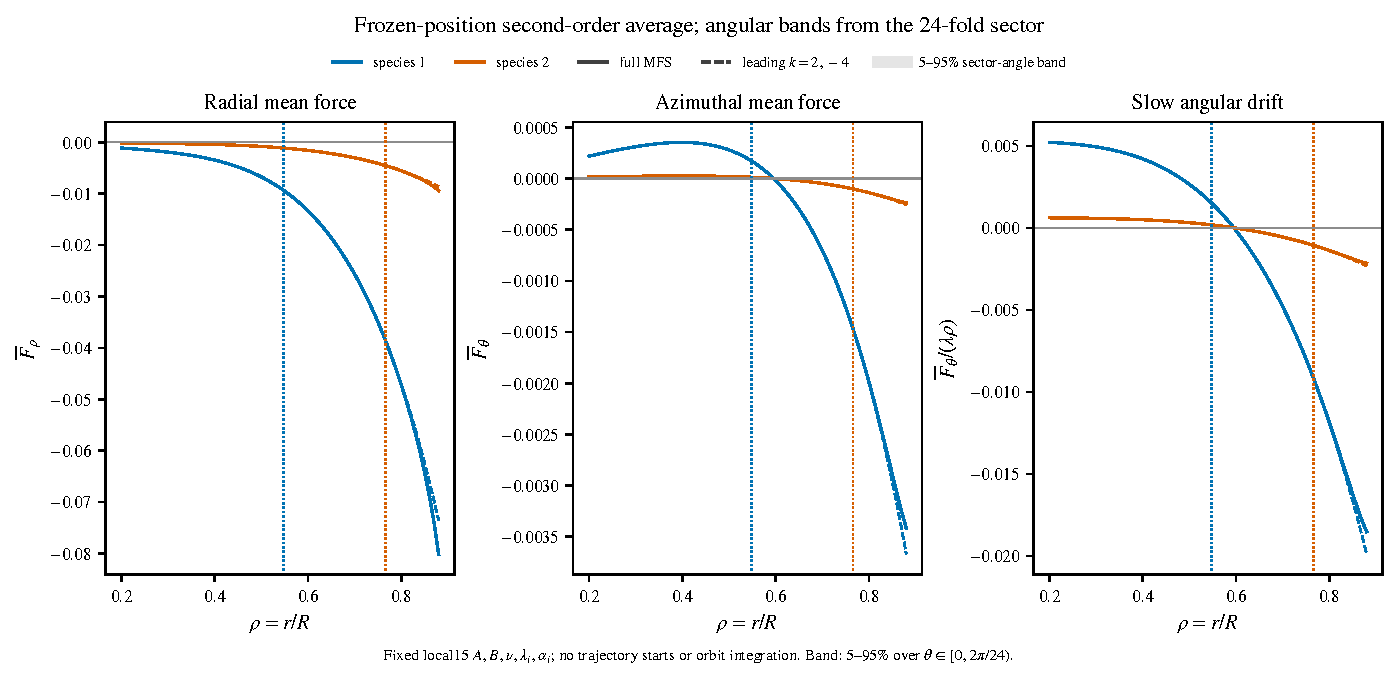
\includegraphics[width=\linewidth]{figures/FIG02_AVERAGED_RF_FORCE_TORQUE.pdf}
\caption{Leading average versus full-MFS frozen-position average over sector angle.}
\end{figure}
\begin{figure}[ht]
\centering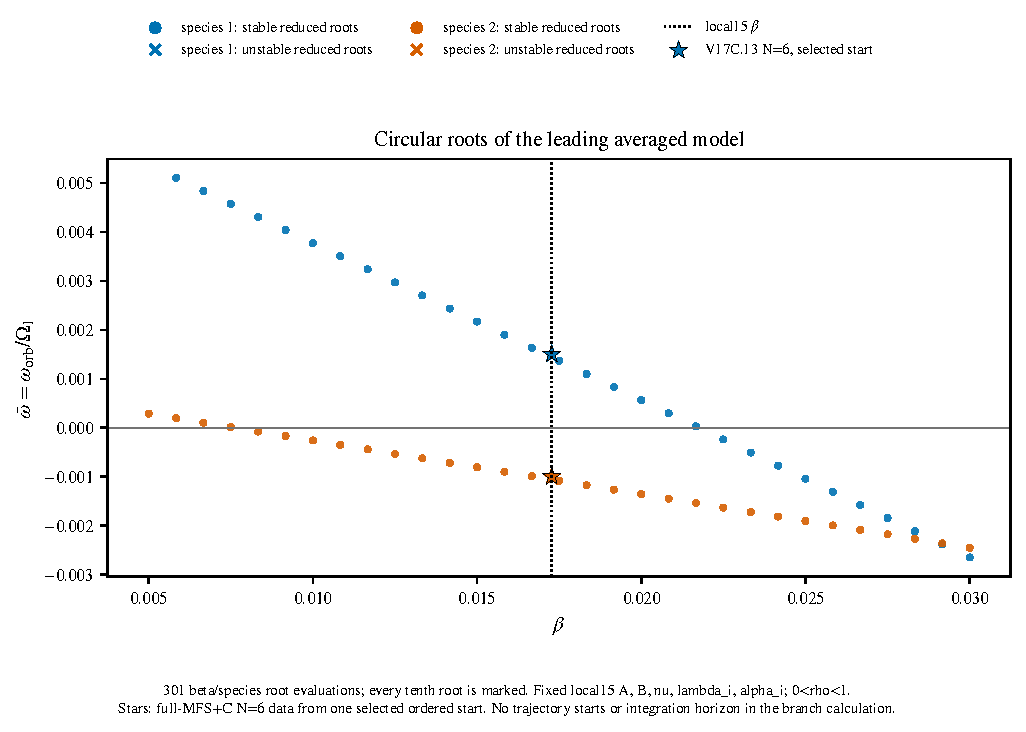
\includegraphics[width=.88\linewidth]{figures/FIG03_ROTATIONAL_BRANCHES.pdf}
\caption{Discrete algebraic circular roots versus \(\beta\); markers classify reduced-model stability, stars show selected full-MFS N=6 means.}
\end{figure}

\section{Момент и коллективные моды}
Точный RF момент на частицу содержит \(-Q_i\partial_{\theta_i}\phi_{\rm RF}\), drag \(-\lambda_iL_i\) и парный Coulomb момент. Для кольца из трёх одинаковых частиц аналитическая внутренняя phase-mode частота равна
\begin{equation}
\omega_C^2=\frac{5\kappa Q^2}{4\sqrt3\,\mu\rho^3},\qquad
s_\pm=-\lambda/2\pm\sqrt{\lambda^2/4-\omega_C^2}.
\end{equation}
При локальных local15 параметрах \(\omega_C/\lambda\simeq0.0174\) и \(0.0180\) при \(C=C_0\); isolated-ring приближение остаётся overdamped до \(12C_0\). RF- и inter-ring моды не включены.

Для квадратного DC-поля осевые возмущения 3+3 планарной конфигурации имеют матрицу коэффициентов с Coulomb расстояниями, зависящими от относительной фазы. Frozen-phase Hessian остаётся положительным на исследованном фазовом секторе, но это не Floquet/Lyapunov тест. Гармоника четвёртого порядка
\begin{equation}
H_4=\zeta^4-3\rho^2\zeta^2+\frac38\rho^4
\end{equation}
даёт локальные осевые extremum при \(\zeta_*^2=3\rho^2/2-\beta_2/(2\beta_4)\). Для local15 фиксированных радиусов окно \(0.56799<\beta_4/\beta_2<1.10987\) сохраняет внутреннюю центральную кривизну и создаёт внешние off-axis точки. Реальная радиальная и осевая устойчивость не проверена.

\begin{figure}[ht]
\centering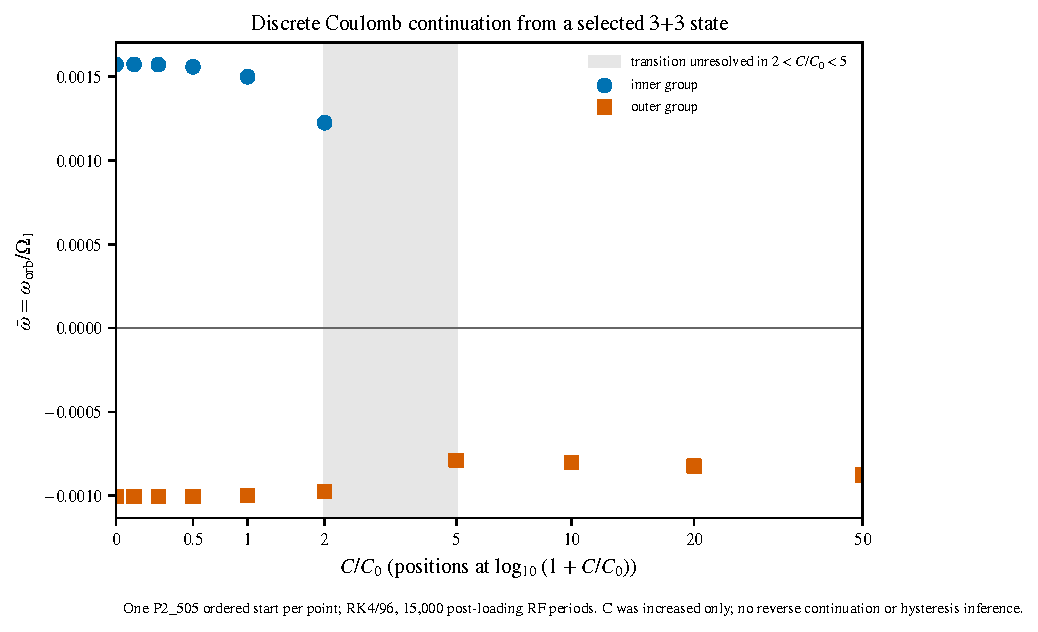
\includegraphics[width=.9\linewidth]{figures/FIG04_COULOMB_ROTATIONAL_TRANSITION.pdf}
\caption{One-way, one-start Coulomb sweep. The sign change is bracketed between \(2\) and \(5\); this is not a basin probability or hysteresis loop.}
\end{figure}
\begin{figure}[ht]
\centering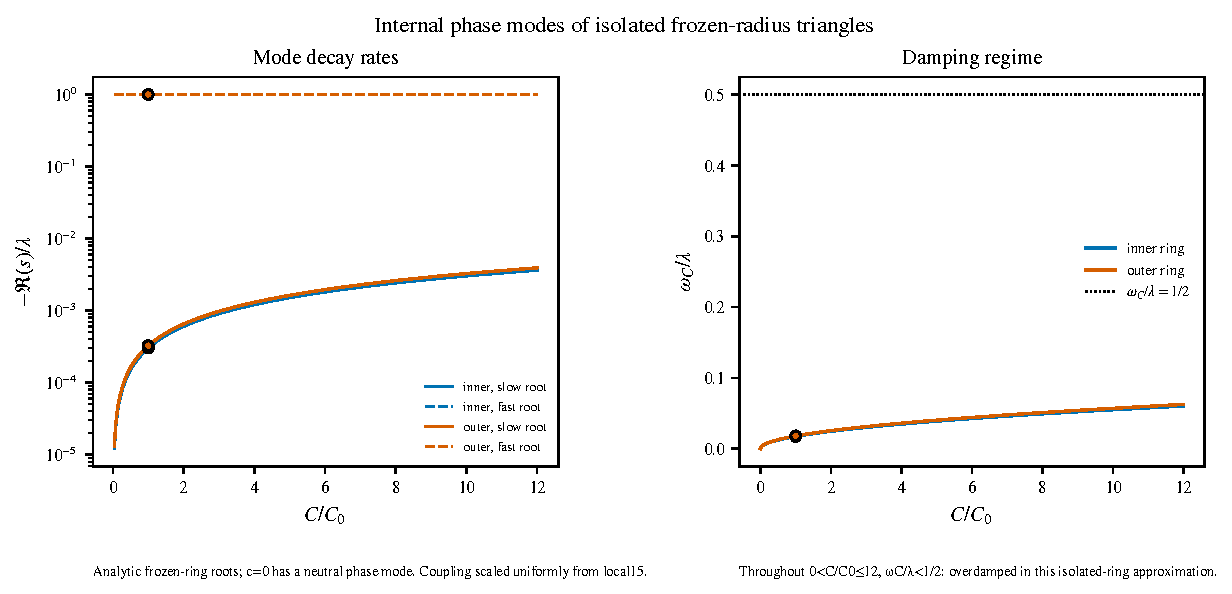
\includegraphics[width=.94\linewidth]{figures/FIG05_INTERNAL_PHASE_MODE_SPECTRUM.pdf}
\caption{Isolated frozen-radius triangular-ring internal phase-mode approximation.}
\end{figure}
\begin{figure}[ht]
\centering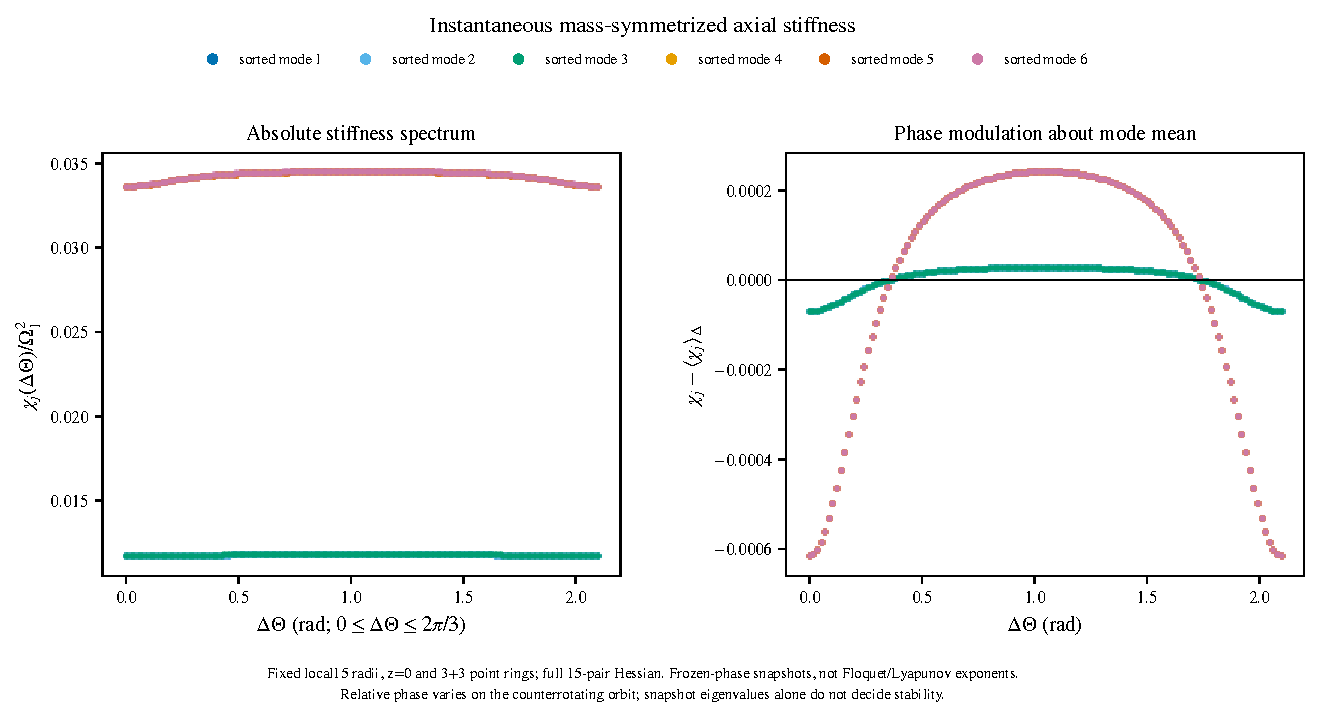
\includegraphics[width=.98\linewidth]{figures/FIG06_AXIAL_COLLECTIVE_STIFFNESS.pdf}
\caption{Instantaneous 3+3 axial stiffness snapshots as relative phase varies; not Floquet exponents.}
\end{figure}
\begin{figure}[ht]
\centering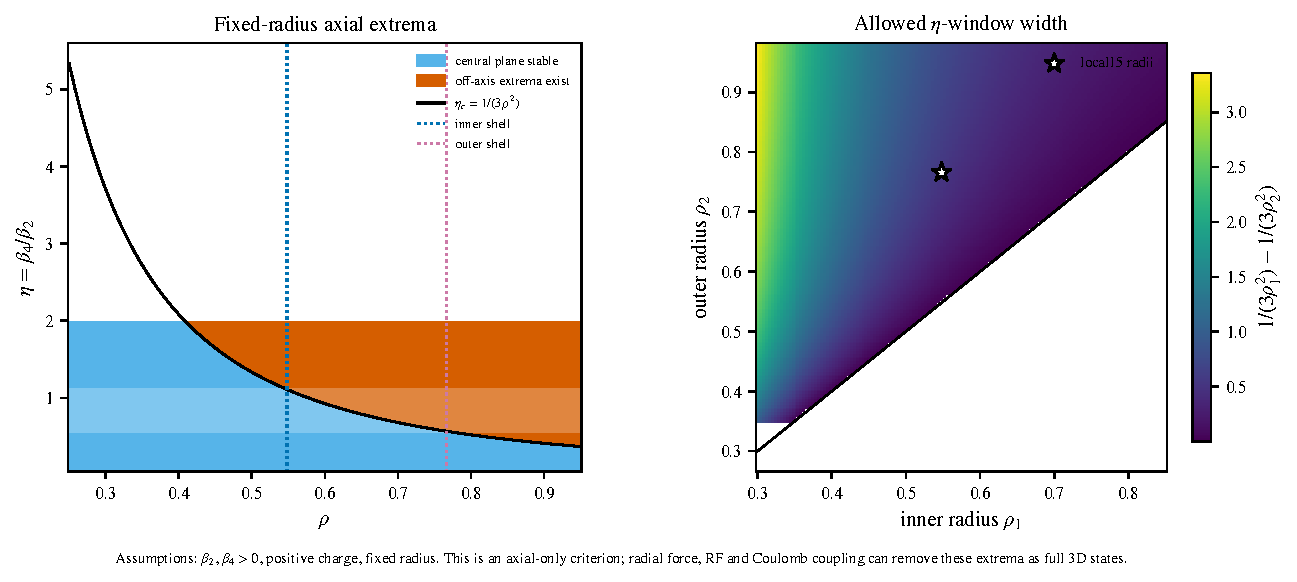
\includegraphics[width=.96\linewidth]{figures/FIG07_H4_AXIAL_STABILITY_MAP.pdf}
\caption{Fixed-radius axial-extrema criteria for the Laplace-compatible \(H_2+H_4\) potential.}
\end{figure}
\begin{figure}[ht]
\centering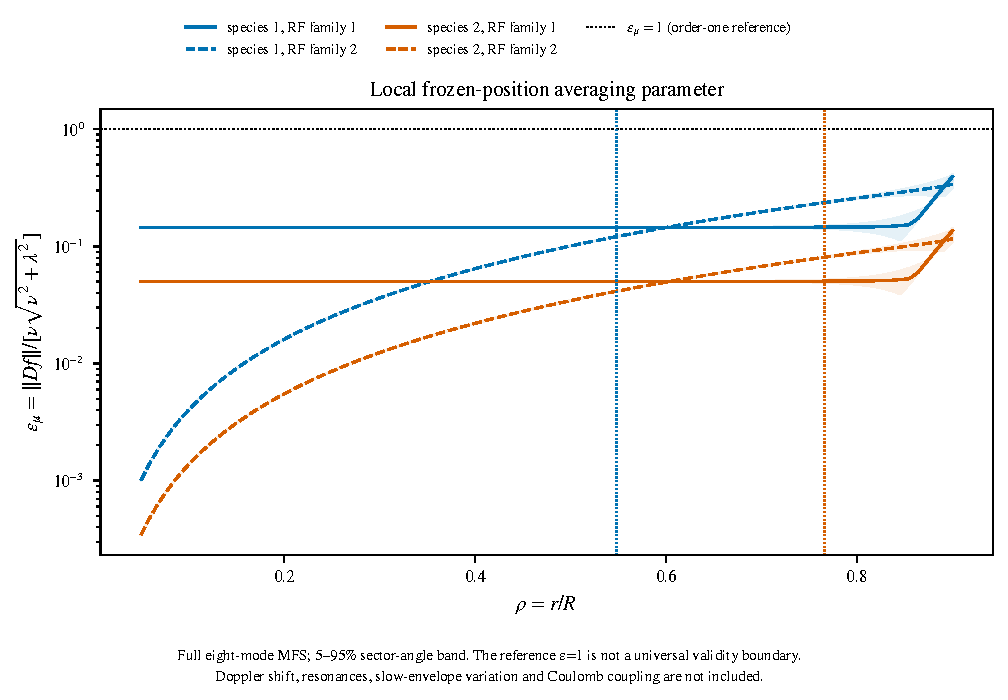
\includegraphics[width=.87\linewidth]{figures/FIG08_AVERAGING_VALIDITY.pdf}
\caption{Local frozen-position micromotion correction indicator; \(\epsilon_\mu=1\) is only an order-one reference.}
\end{figure}

\section{Проверки и пределы утверждений}
Пять тестов RHS/Jacobian прошли; фазовая квадратура локального среднего согласуется с комплексной формулой до \(1.5\times10^{-14}\), leading-mode formula до \(1.1\times10^{-15}\). Эти величины не измеряют точность орбитального усреднения. Новые интегрирования траекторий, случайные старты, RK4 step refinement, DOP853, обратное continuation и полный tangent/Floquet-Lyapunov расчёт не выполнялись. Размеры, заряд, пробой, газовая среда и drag не получили независимой физической квалификации в V17C.14. Рисунки должны читаться вместе с `FIGURE_AUDIT_RU.md` и `NUMERICAL_VALIDATION_RU.md`.

RF-trap micromotion and Floquet theory are discussed in \cite{Dehmelt1967Storage,Landa2012Modes,Kaufmann2012Eigenmodes}; Coulomb structural transitions in \cite{Dubin1993Structural,Fishman2008Structural}. Rotating-wall Penning plasma experiments \cite{Huang1997Steady,Huang1998PhaseLocked} are contextual analogies only.

\bibliographystyle{unsrt}
\bibliography{references}
\end{document}
